\documentclass[12pt,a4paper,article,english,firamath]{nsi}
\pagestyle{empty}
\begin{document}
\titre{TP 2 - Chronogrammes}
\classe{NSI2}
\maketitle

\subsection*{Exercice 1}
On considère les processus suivants
\begin{center}
\begin{tabular}{|c|c|c|c|}
\hline\rowcolor{UGLiOrange}
\textbf{\color{white} Processus} & \textbf{\color{white}Départ} & \textbf{\color{white}Durée} & \textbf{\color{white}Priorité} \\
\hline
P1 & 7 & 3 & haute \\
\hline
P2 & 2 & 4 & basse \\
\hline
P3 & 0 & 5 & haute \\
\hline
P4 & 5 & 2 & basse \\
\hline
\end{tabular}
\end{center}
Donner le chronogramme d'exécution des processus et sa projection dans les cas suivants :
\begin{enumerate}
	\item 	L'ordonnanceur utilise un algorithme FIFO sans priorités.
    \begin{center}
    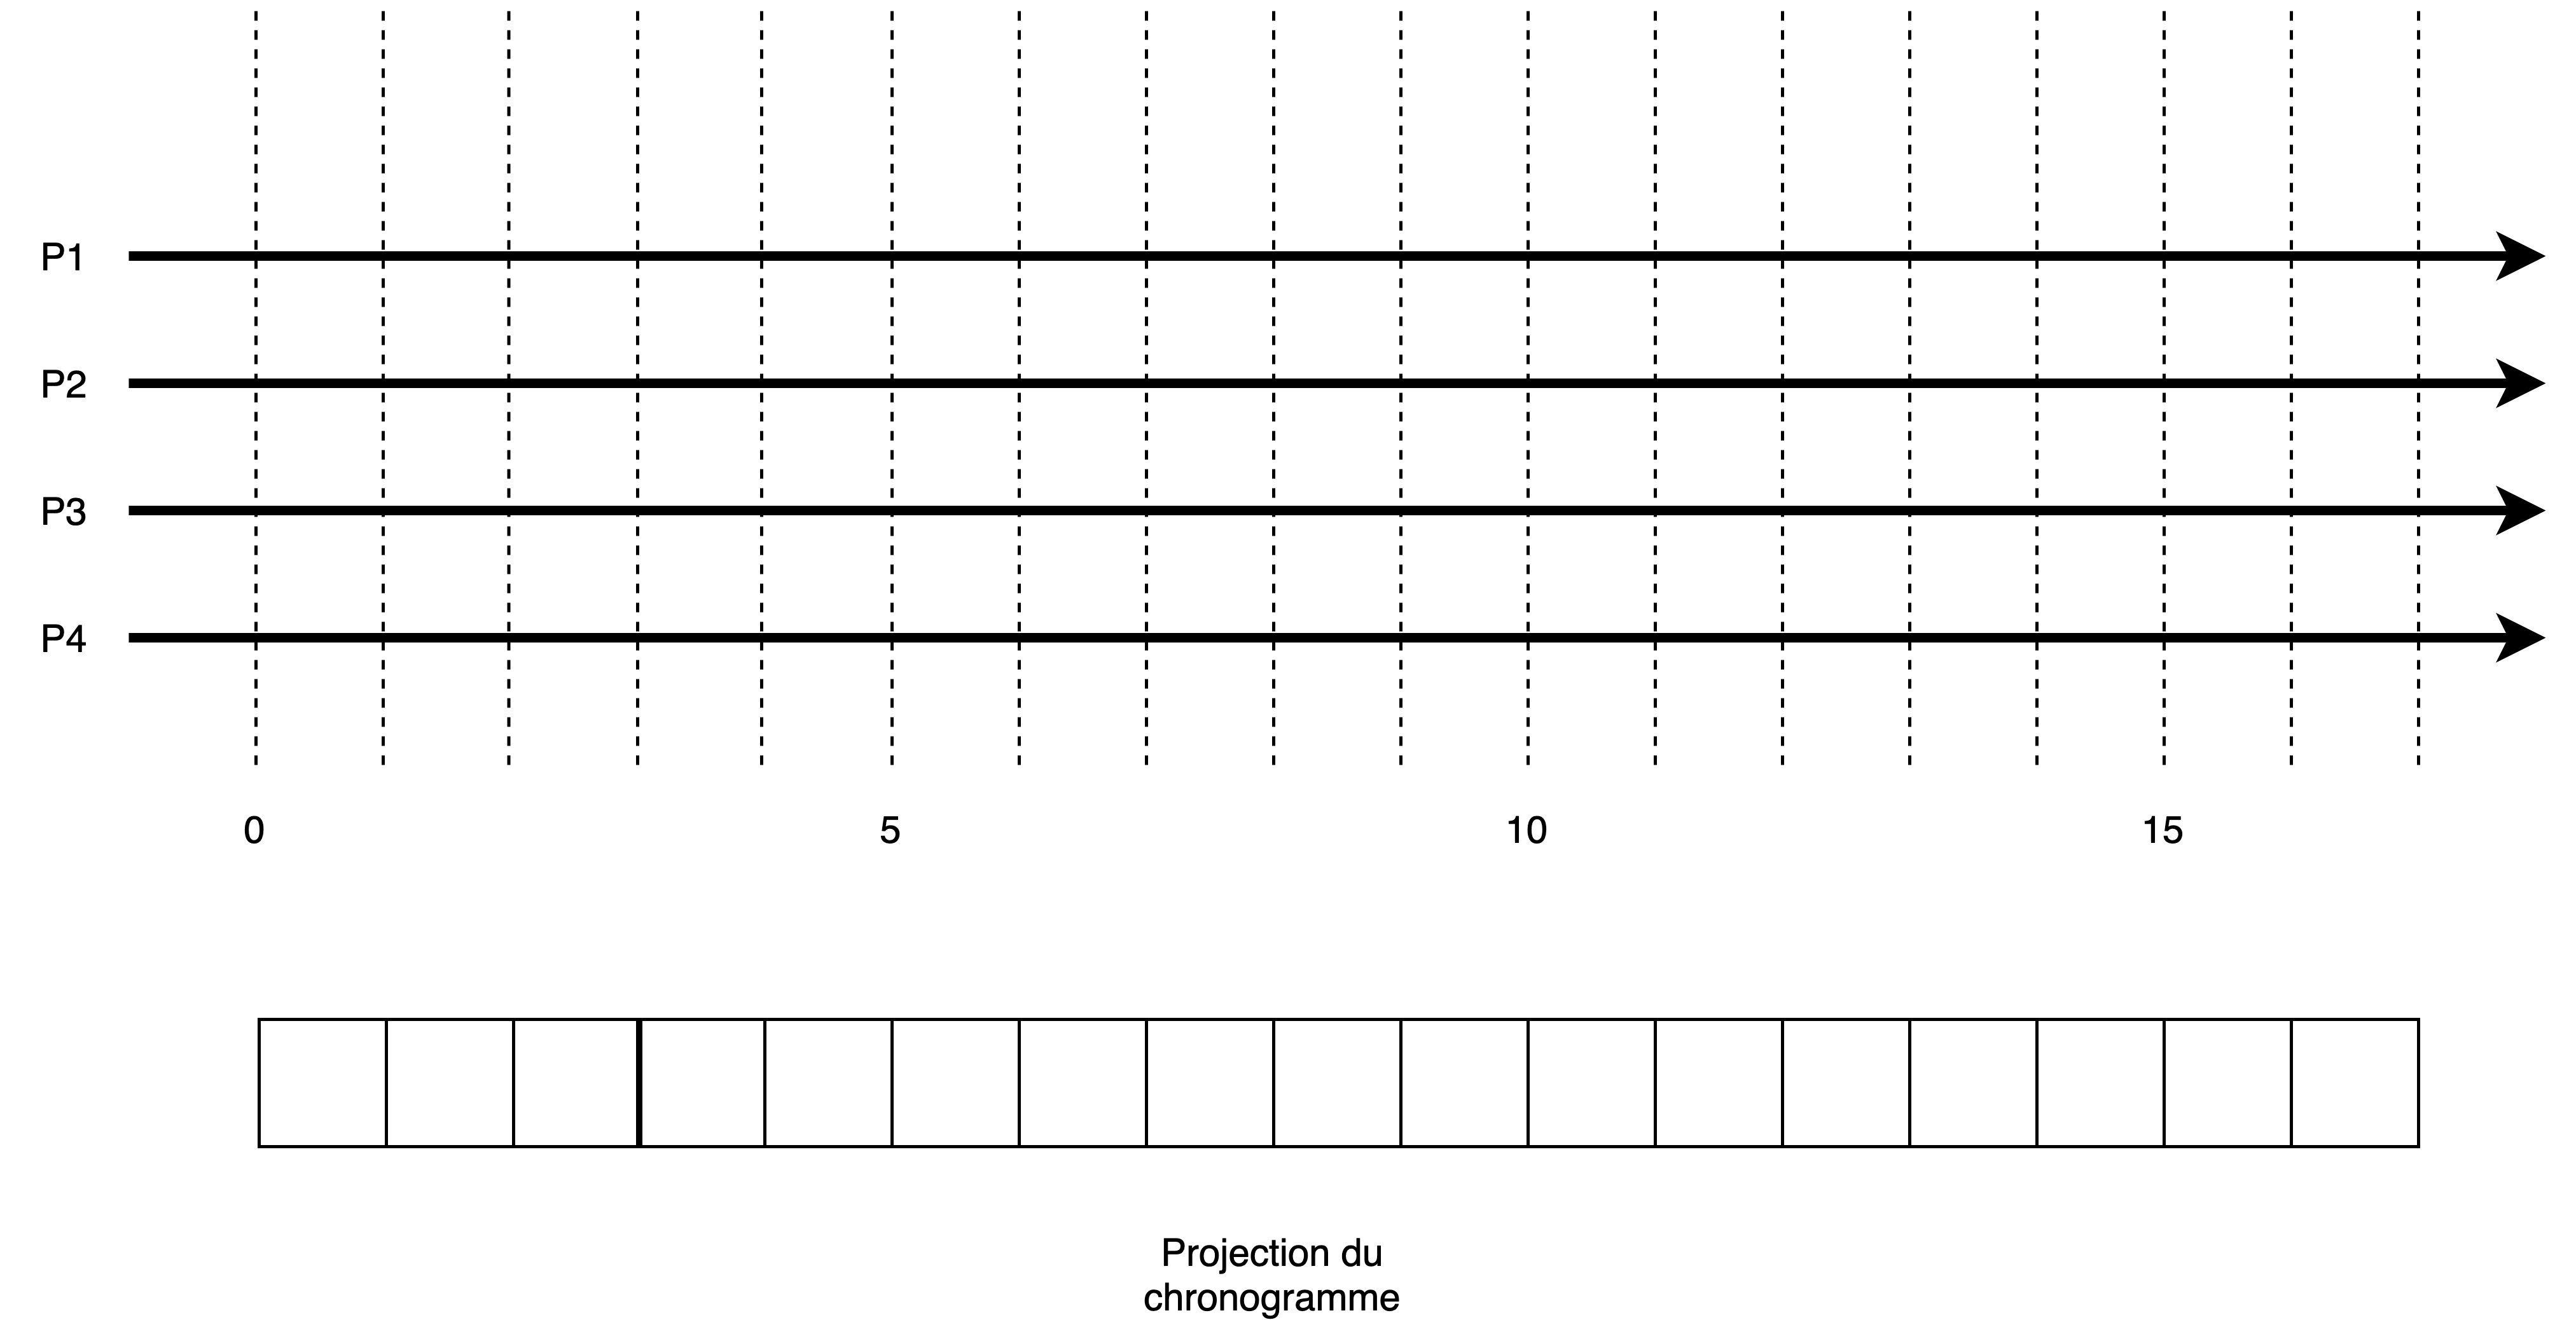
\includegraphics[width=10cm]{img/mc}\\
    \end{center}
	\item 	L'ordonnanceur utilise un algorithme Round Robin sans priorités.
        \begin{center}
        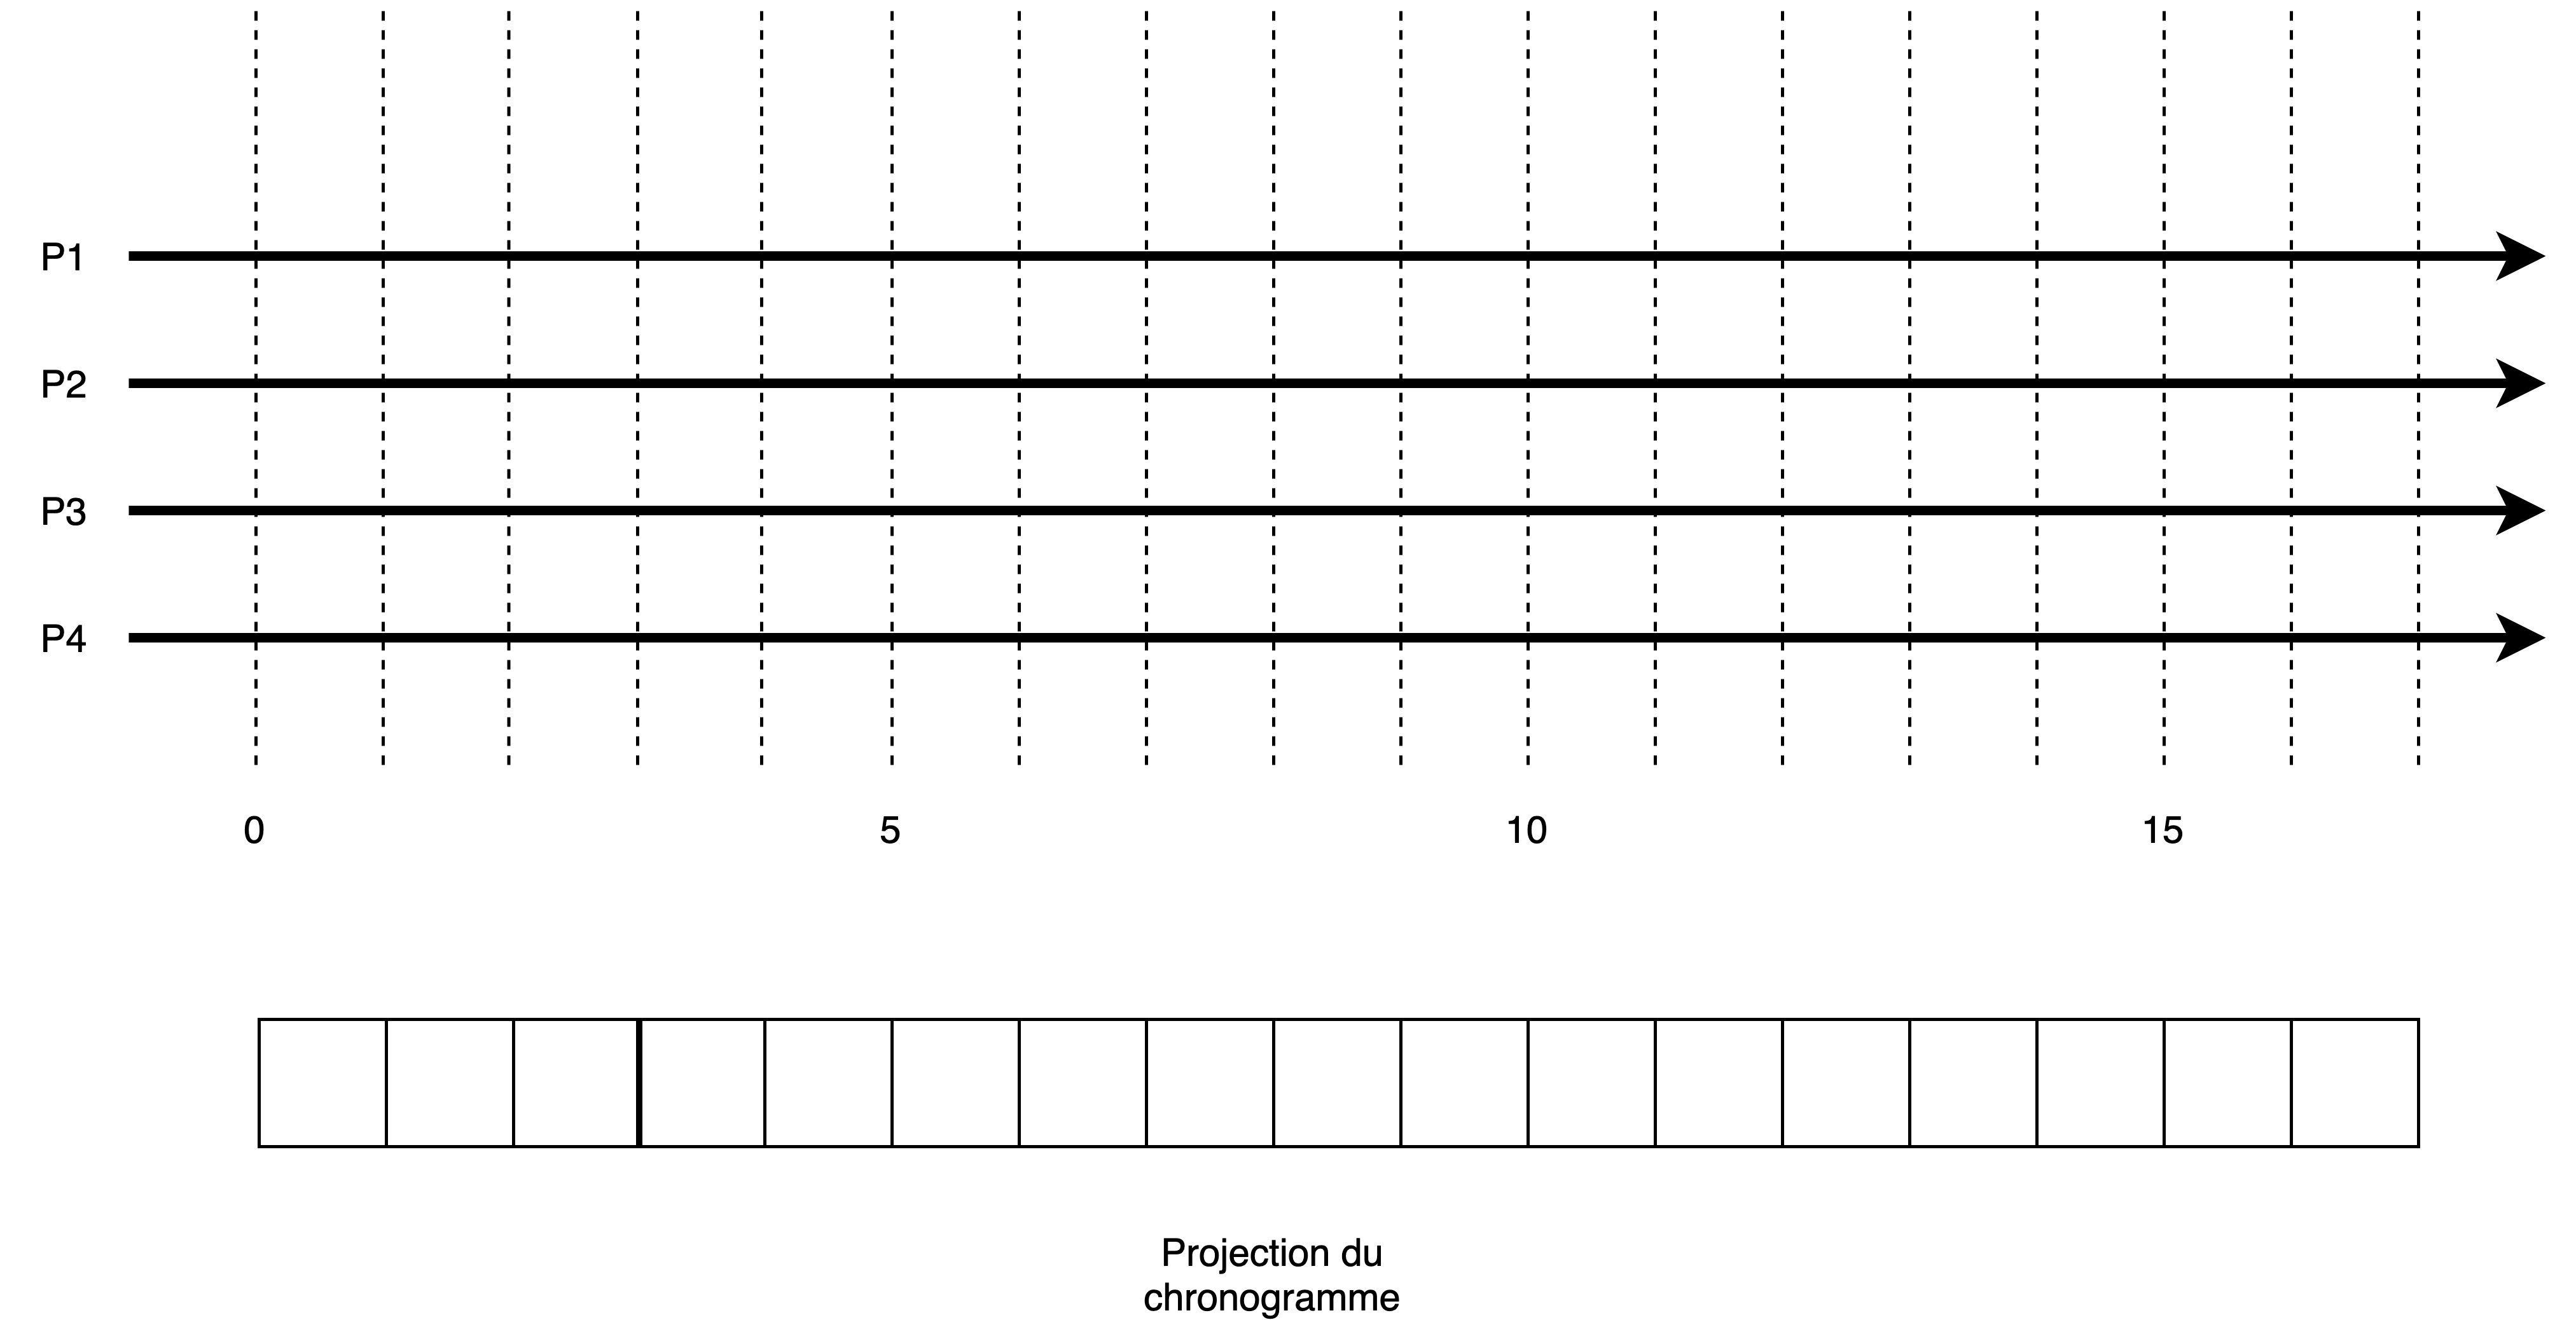
\includegraphics[width=10cm]{img/mc}\\
        \end{center}
        
        \newpage
        
    \item L'ordonnanceur utilise un algorithme FIFO avec priorités.
        \begin{center}
        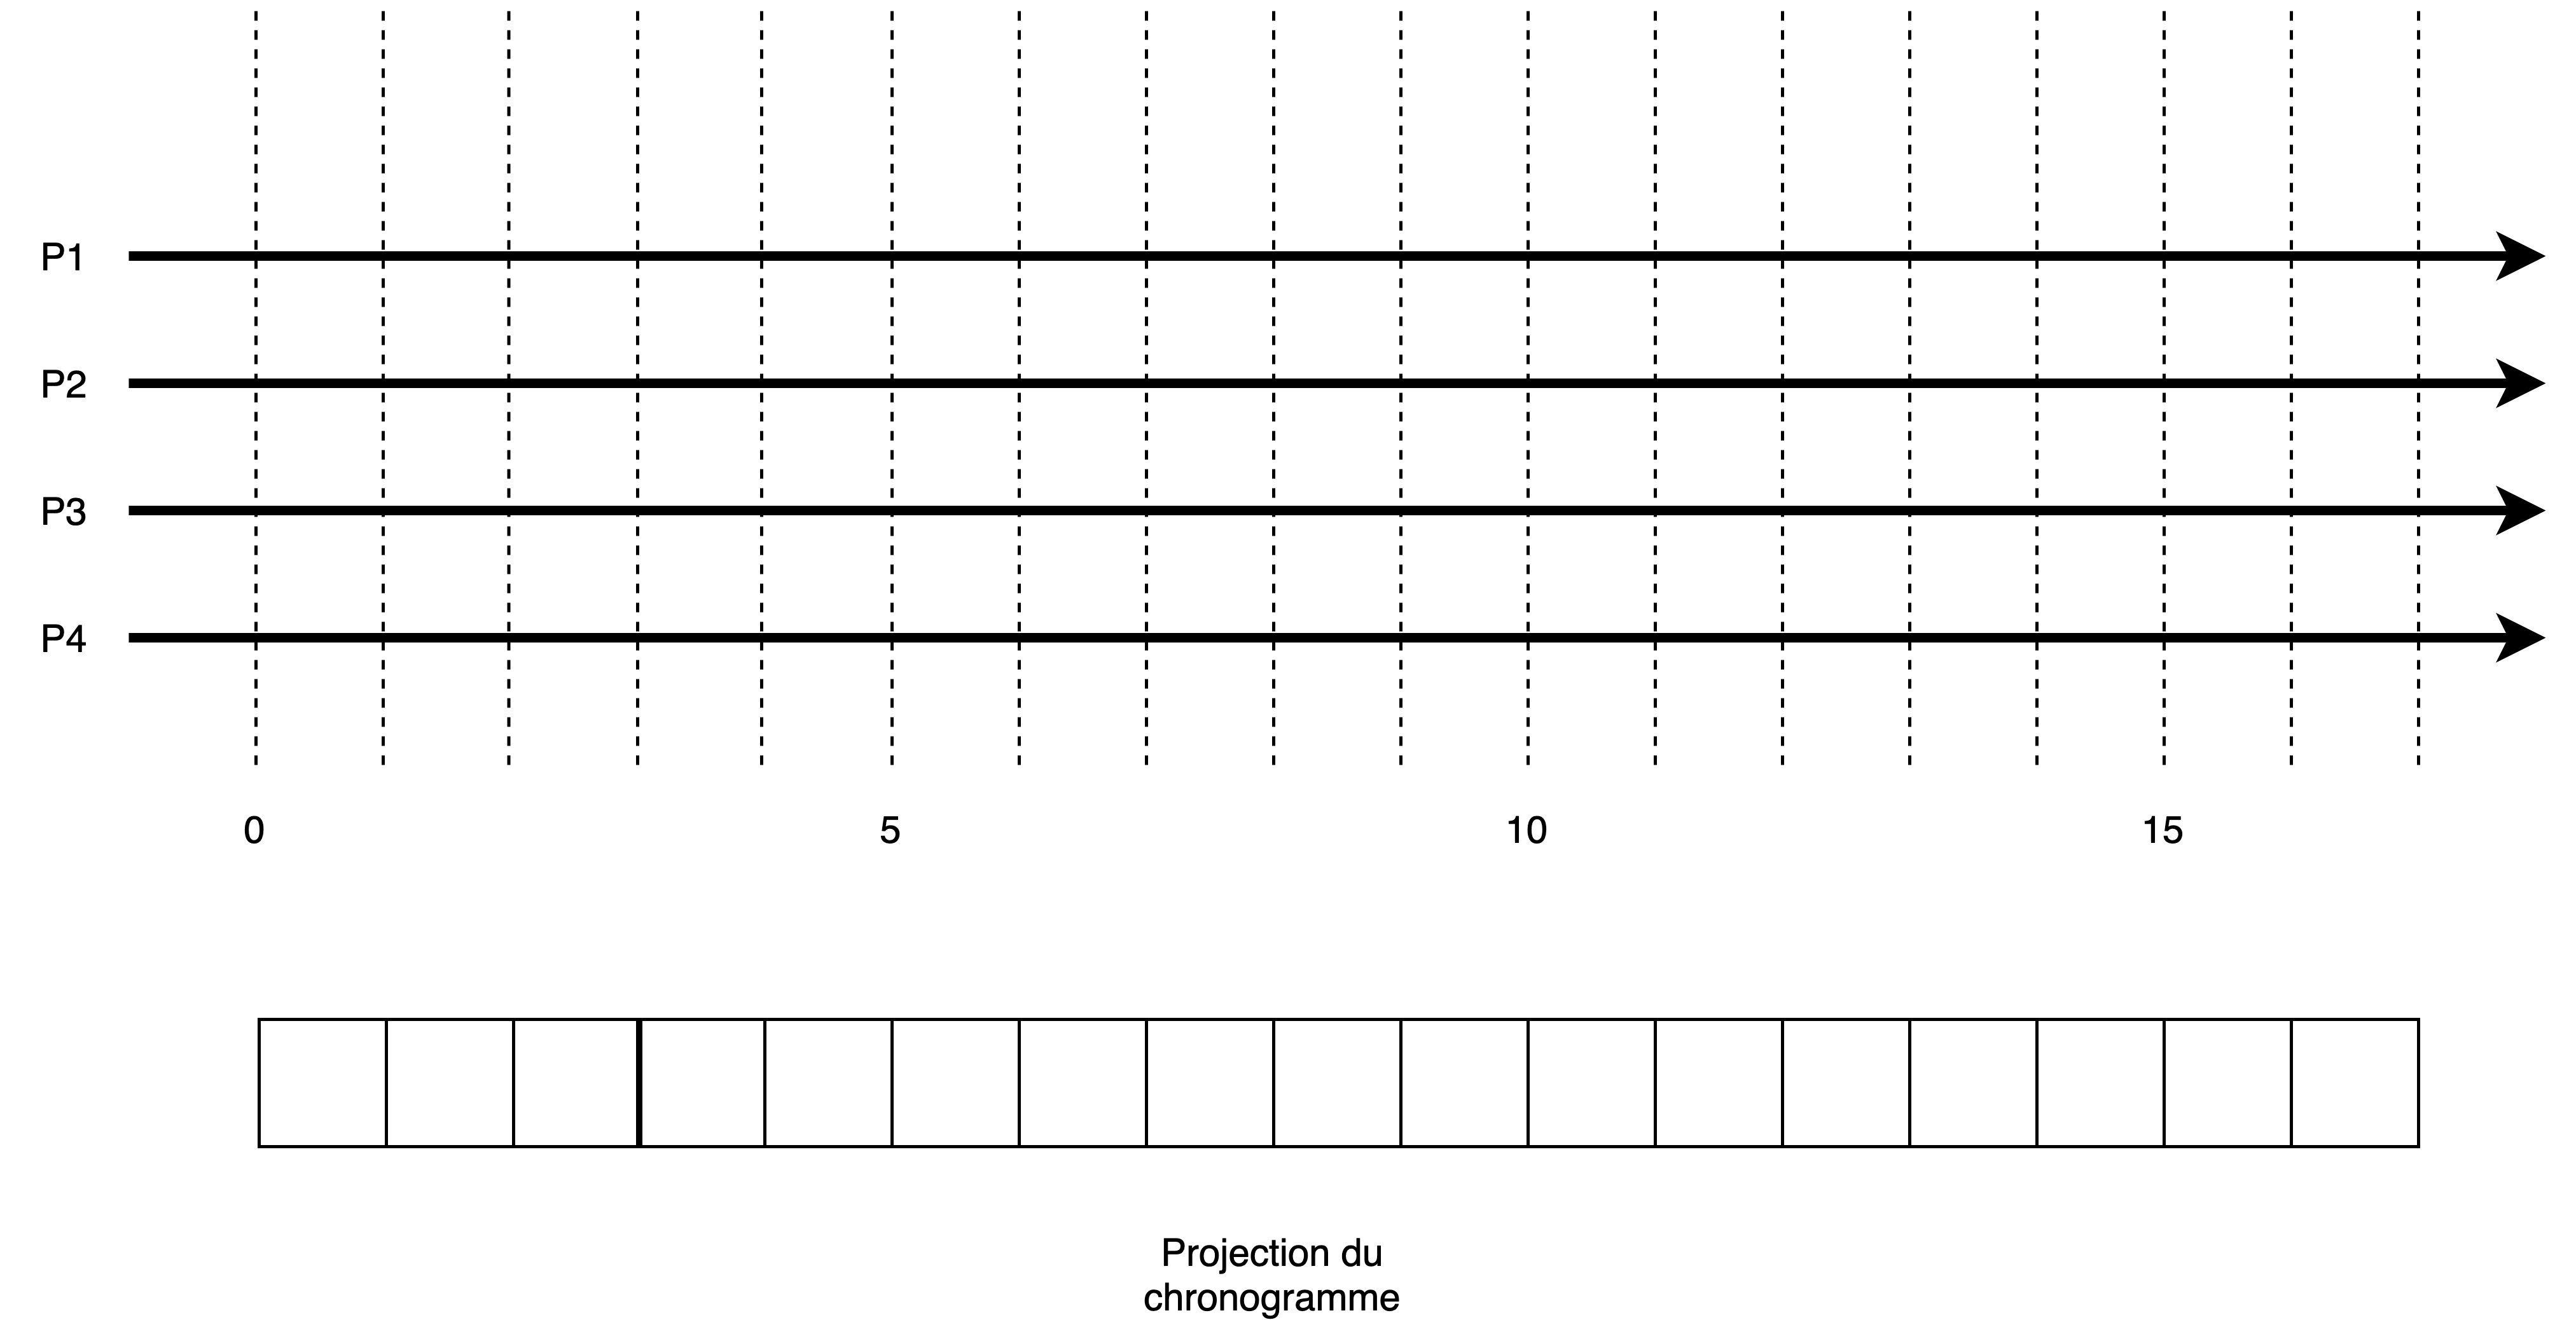
\includegraphics[width=10cm]{img/mc}\\
        \end{center}	
    \item L'ordonnanceur utilise un algorithme Round Robin avec priorités.
        \begin{center}
        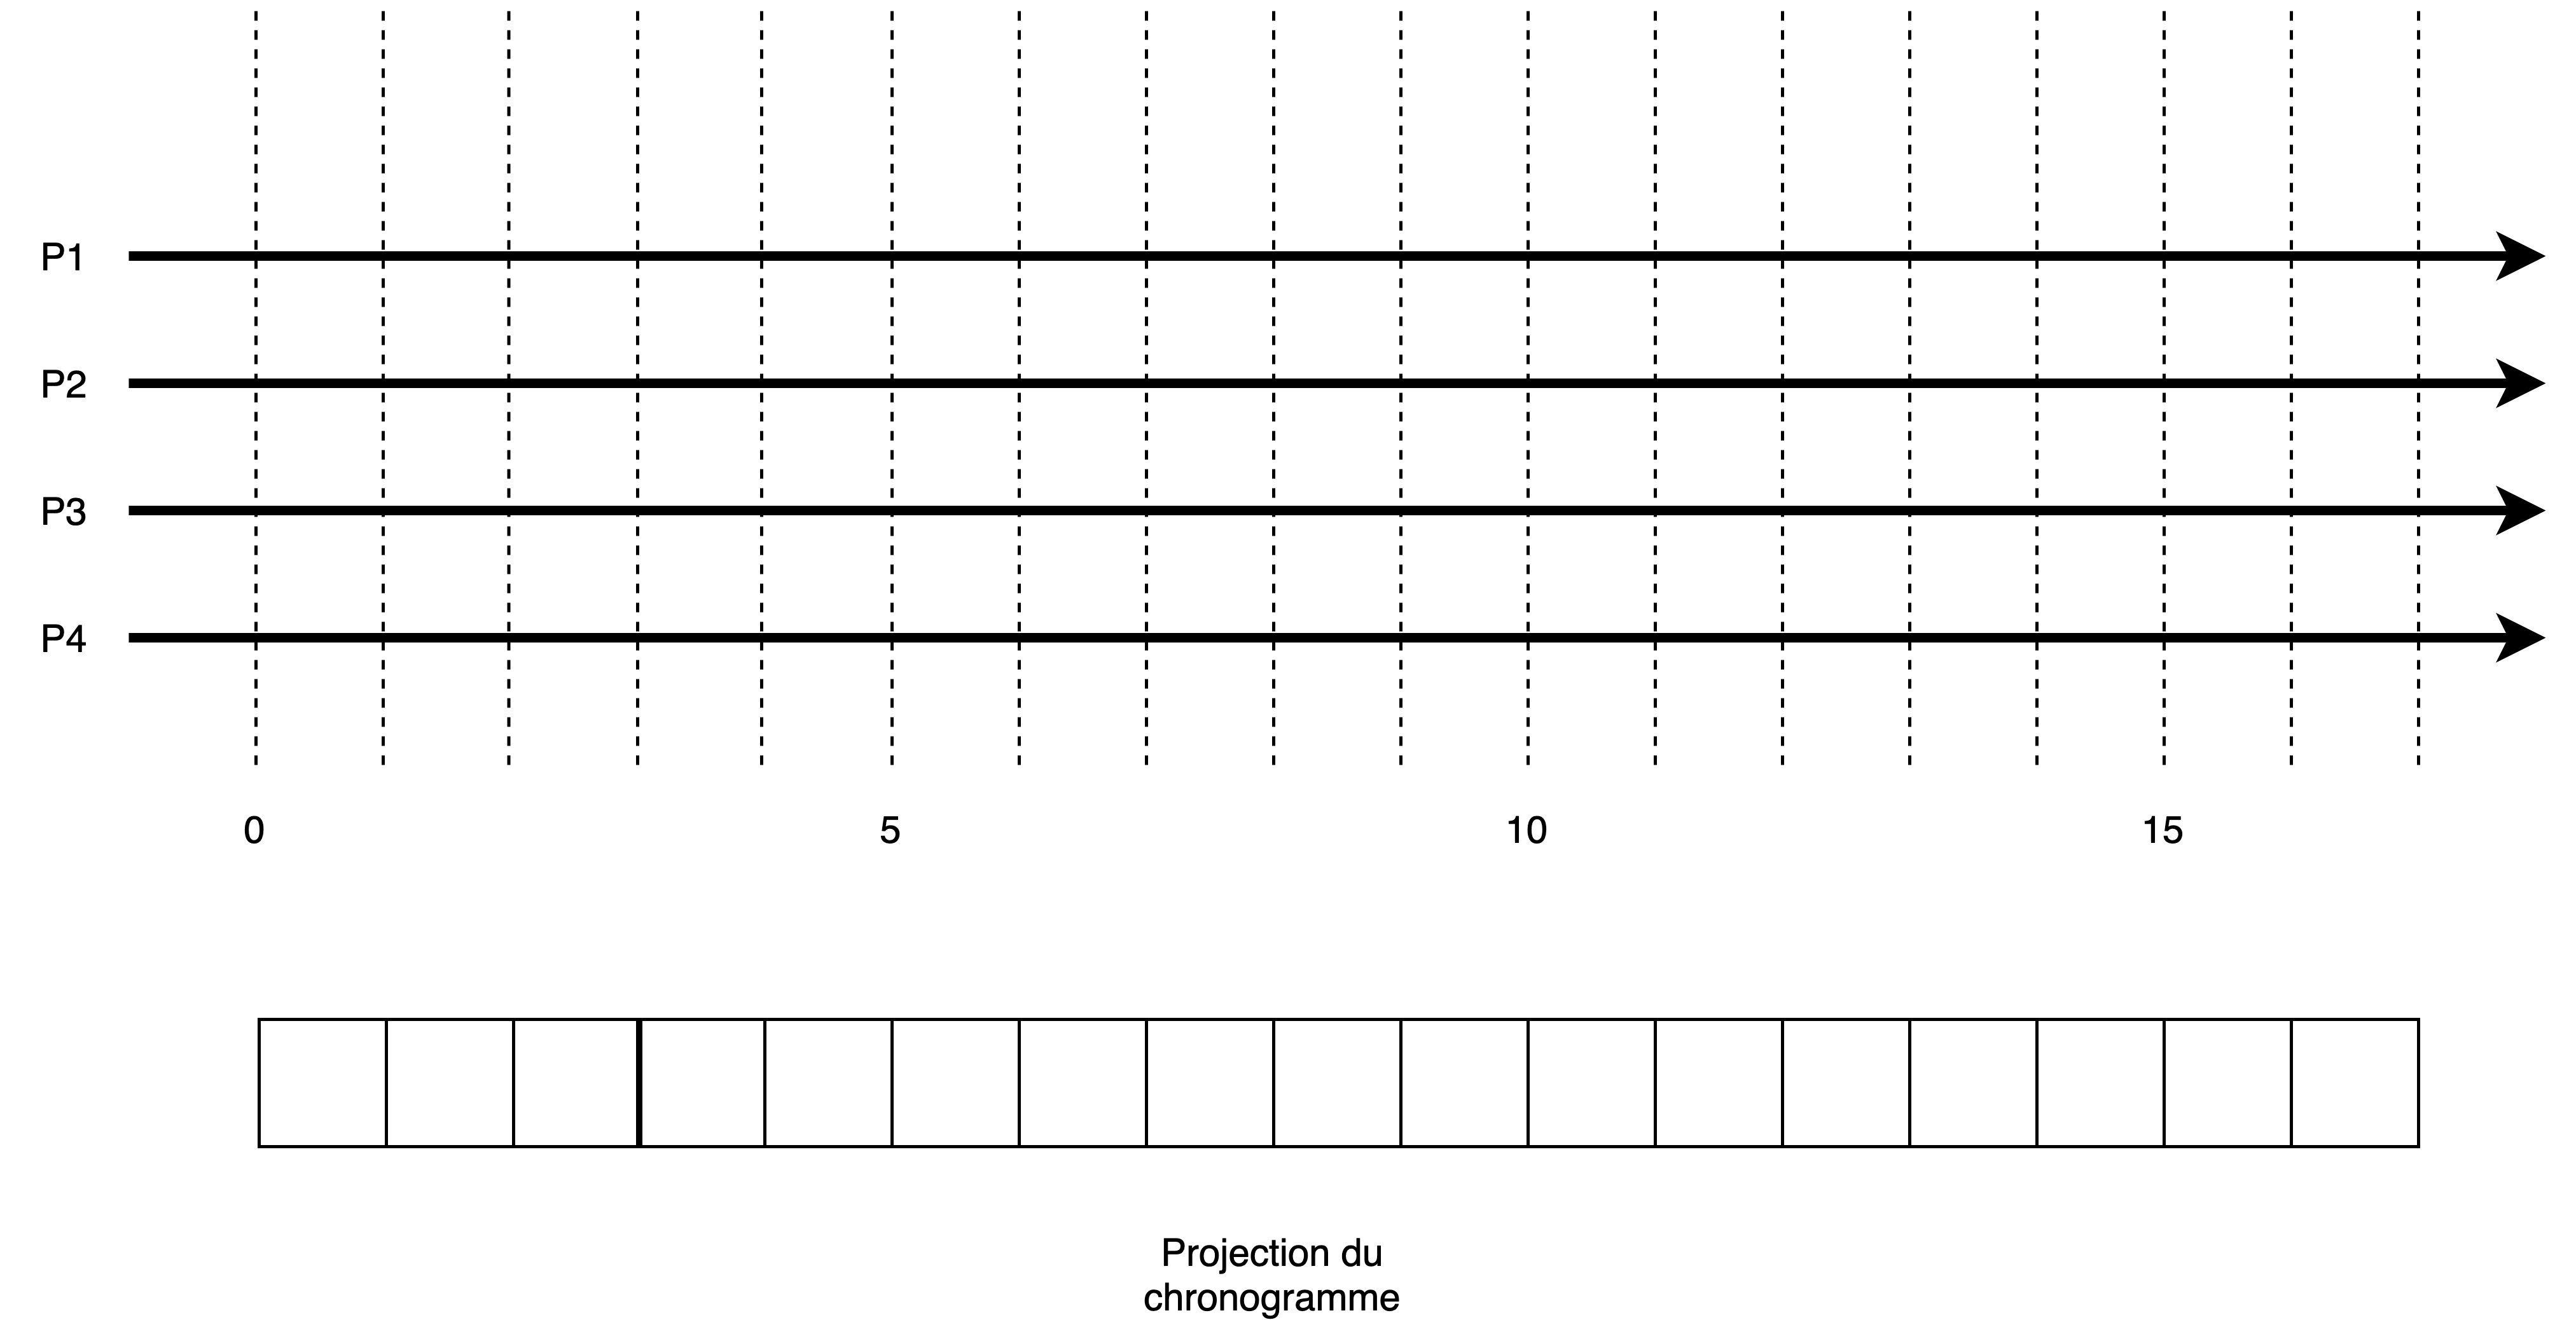
\includegraphics[width=10cm]{img/mc}\\
        \end{center}
        
    \item L'ordonnanceur utilise un algorithme SJF sans priorités.
        \begin{center}
        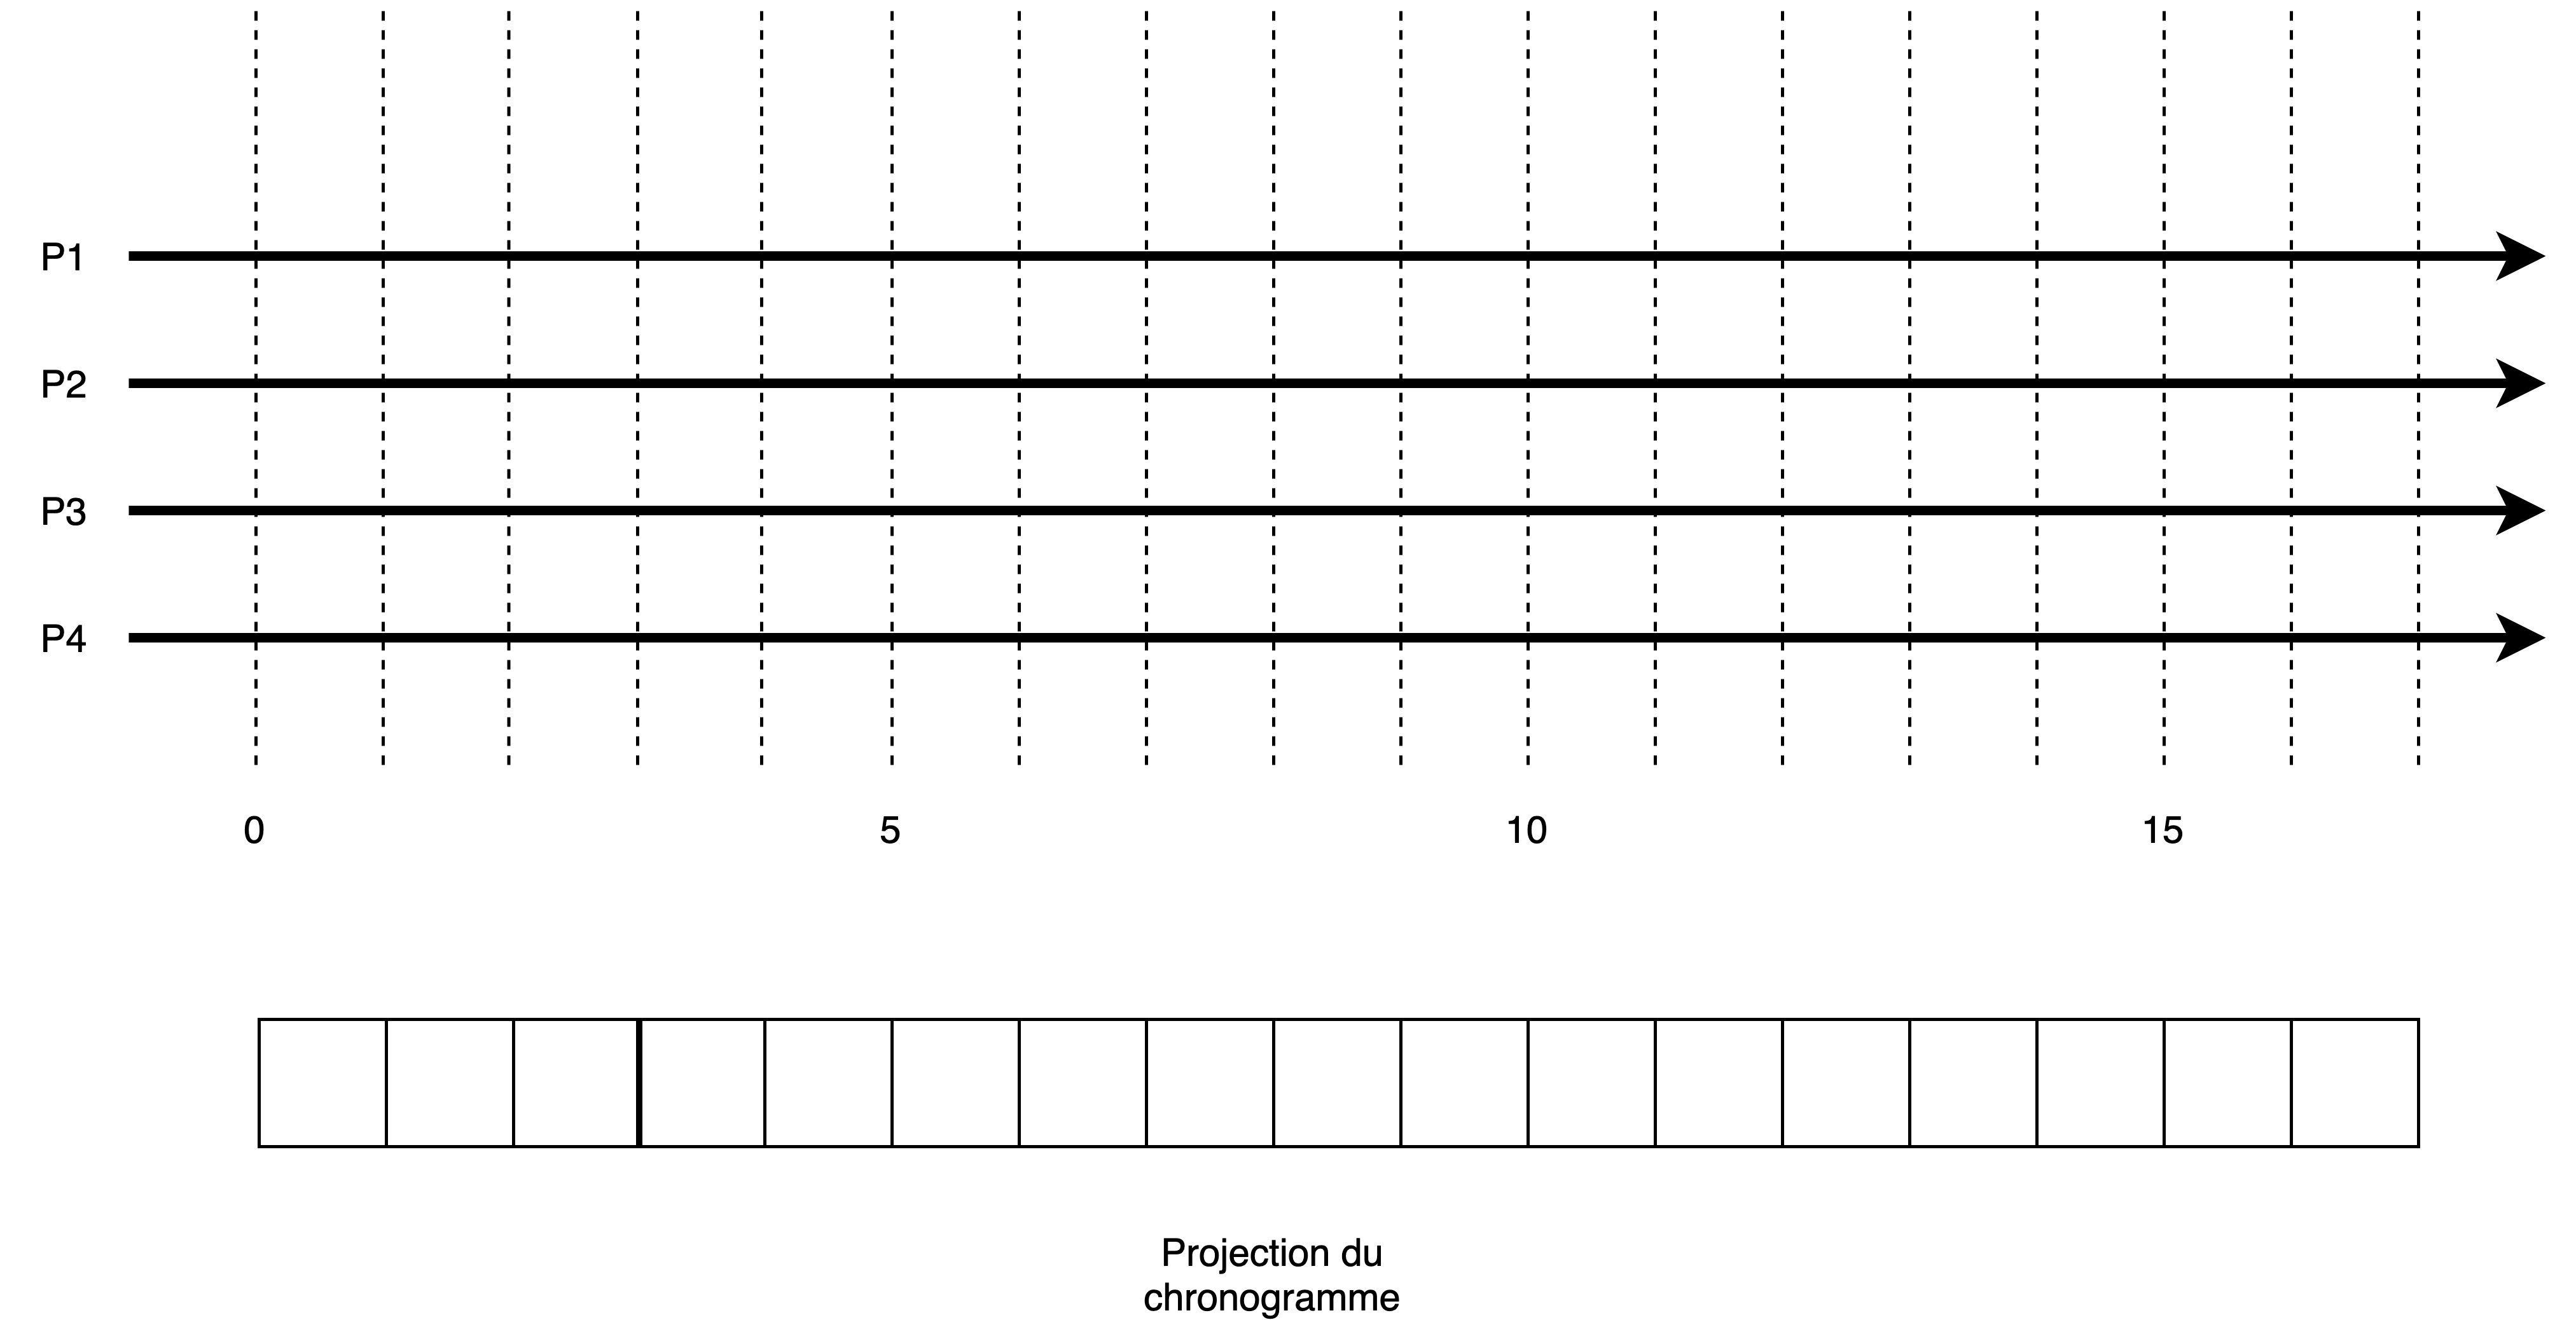
\includegraphics[width=10cm]{img/mc}\\
        \end{center}
    
    \item L'ordonnanceur utilise un algorithme SJF avec priorités.
            \begin{center}
            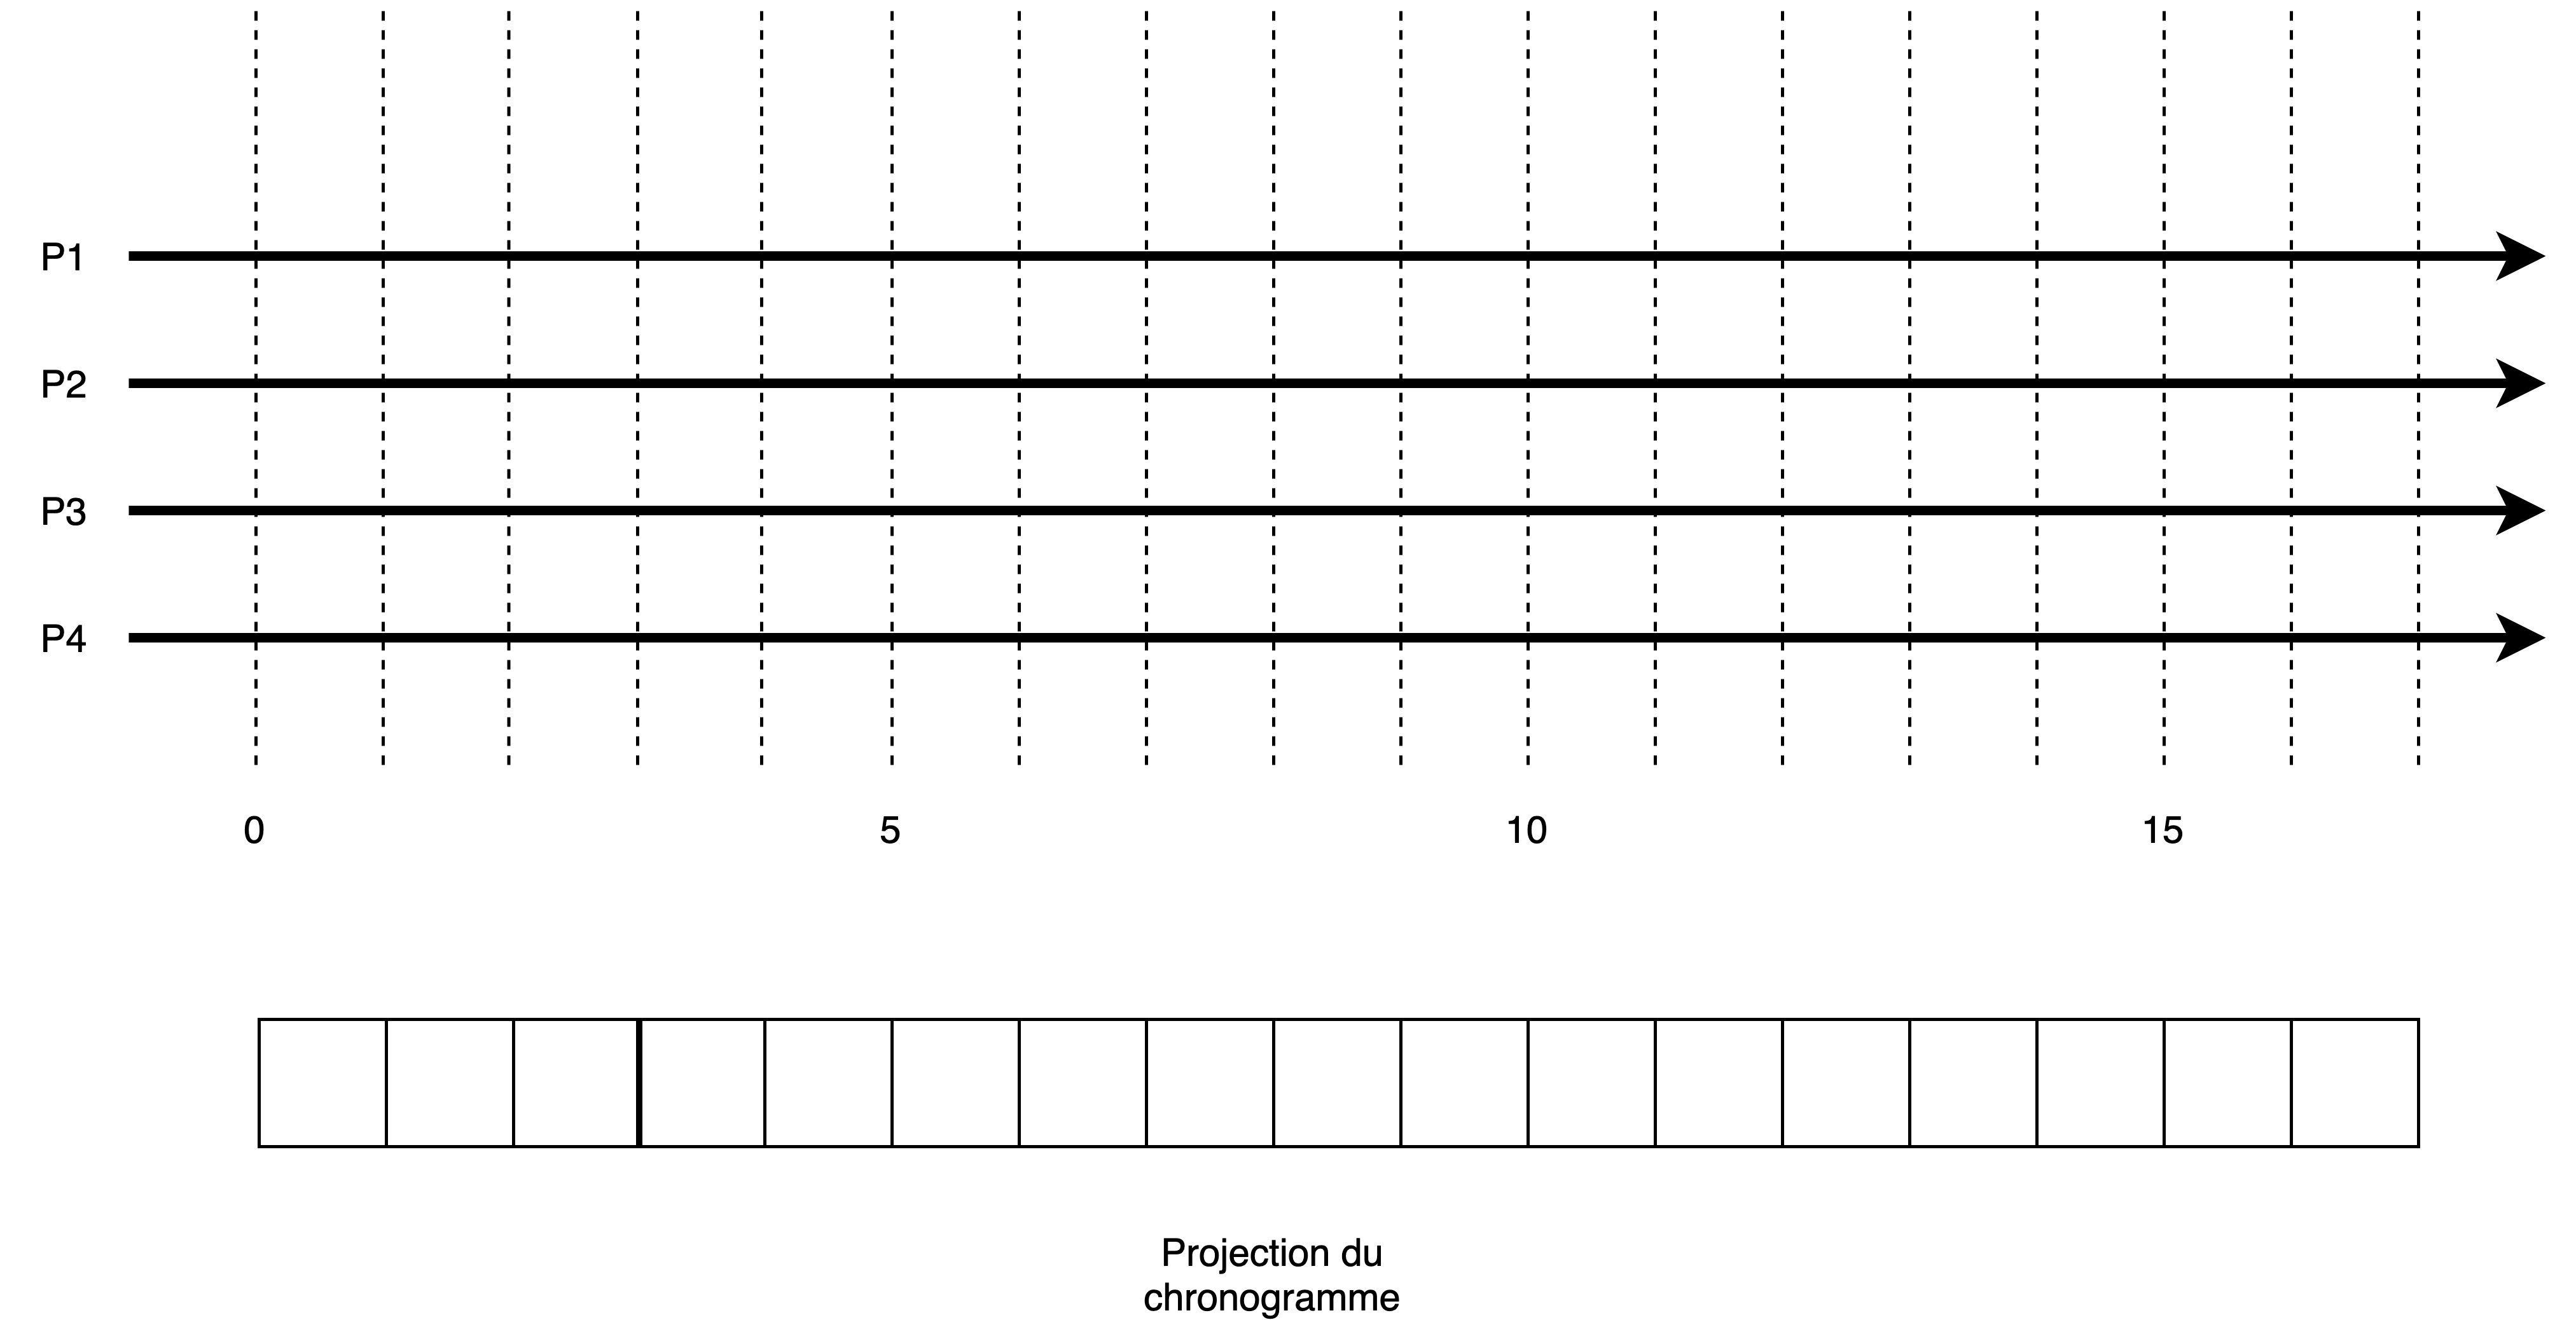
\includegraphics[width=10cm]{img/mc}\\
            \end{center}
        
     \item L'ordonnanceur utilise un algorithme SRJF (\textit{Shortest Remaining Job First}) sans priorités : la tâche élue est celle dont le temps d'exécution \textit{restant} est le plus court.
                 \begin{center}
                 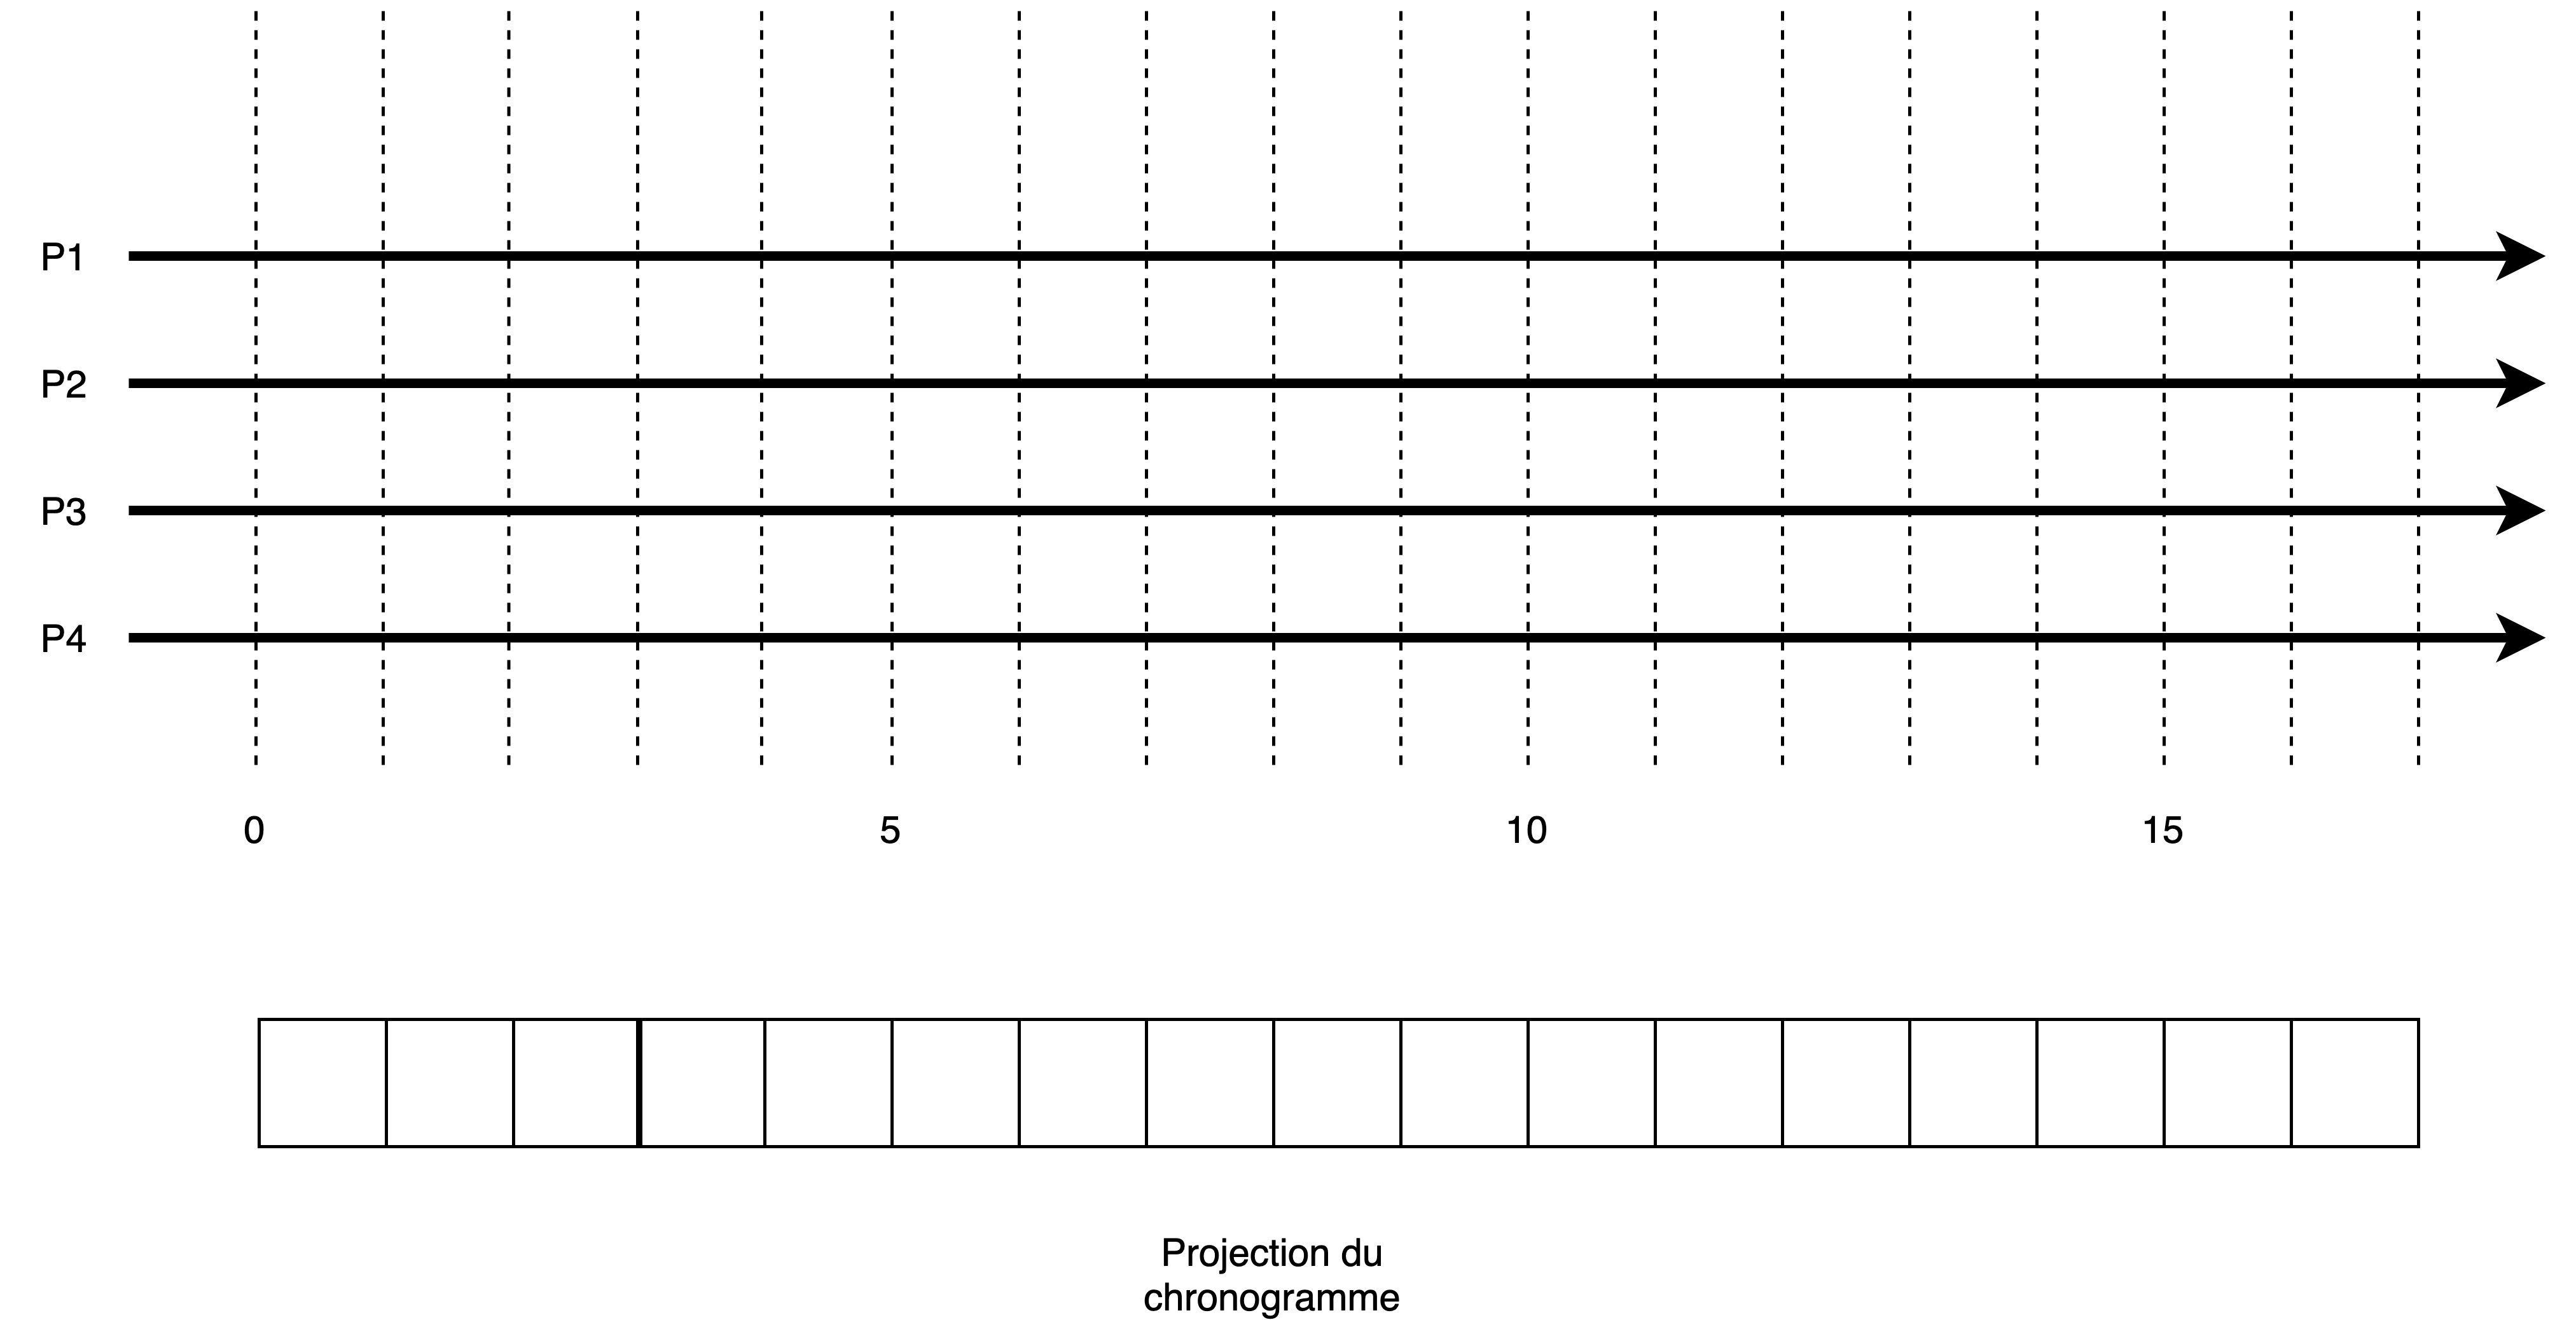
\includegraphics[width=10cm]{img/mc}\\
                 \end{center}
\end{enumerate}

\subsection*{Exercice 2}

On considère les processus suivants
\begin{center}
\begin{tabular}{|c|c|c|}
\hline\rowcolor{UGLiOrange}
\textbf{\color{white} Processus} & \textbf{\color{white}Départ} & \textbf{\color{white}Durée} \\
\hline
P1 & 0 & 3 \\
\hline
P2 & 2 & 2 \\
\hline
P3 & 6 & 2 \\
\hline
P4 & 7 & 3 \\
\hline
\end{tabular}
\end{center}
Donner le chronogramme d'exécution des processus et sa projection dans les cas suivants :
\begin{enumerate}
	\item 	RR.
    \begin{center}
                     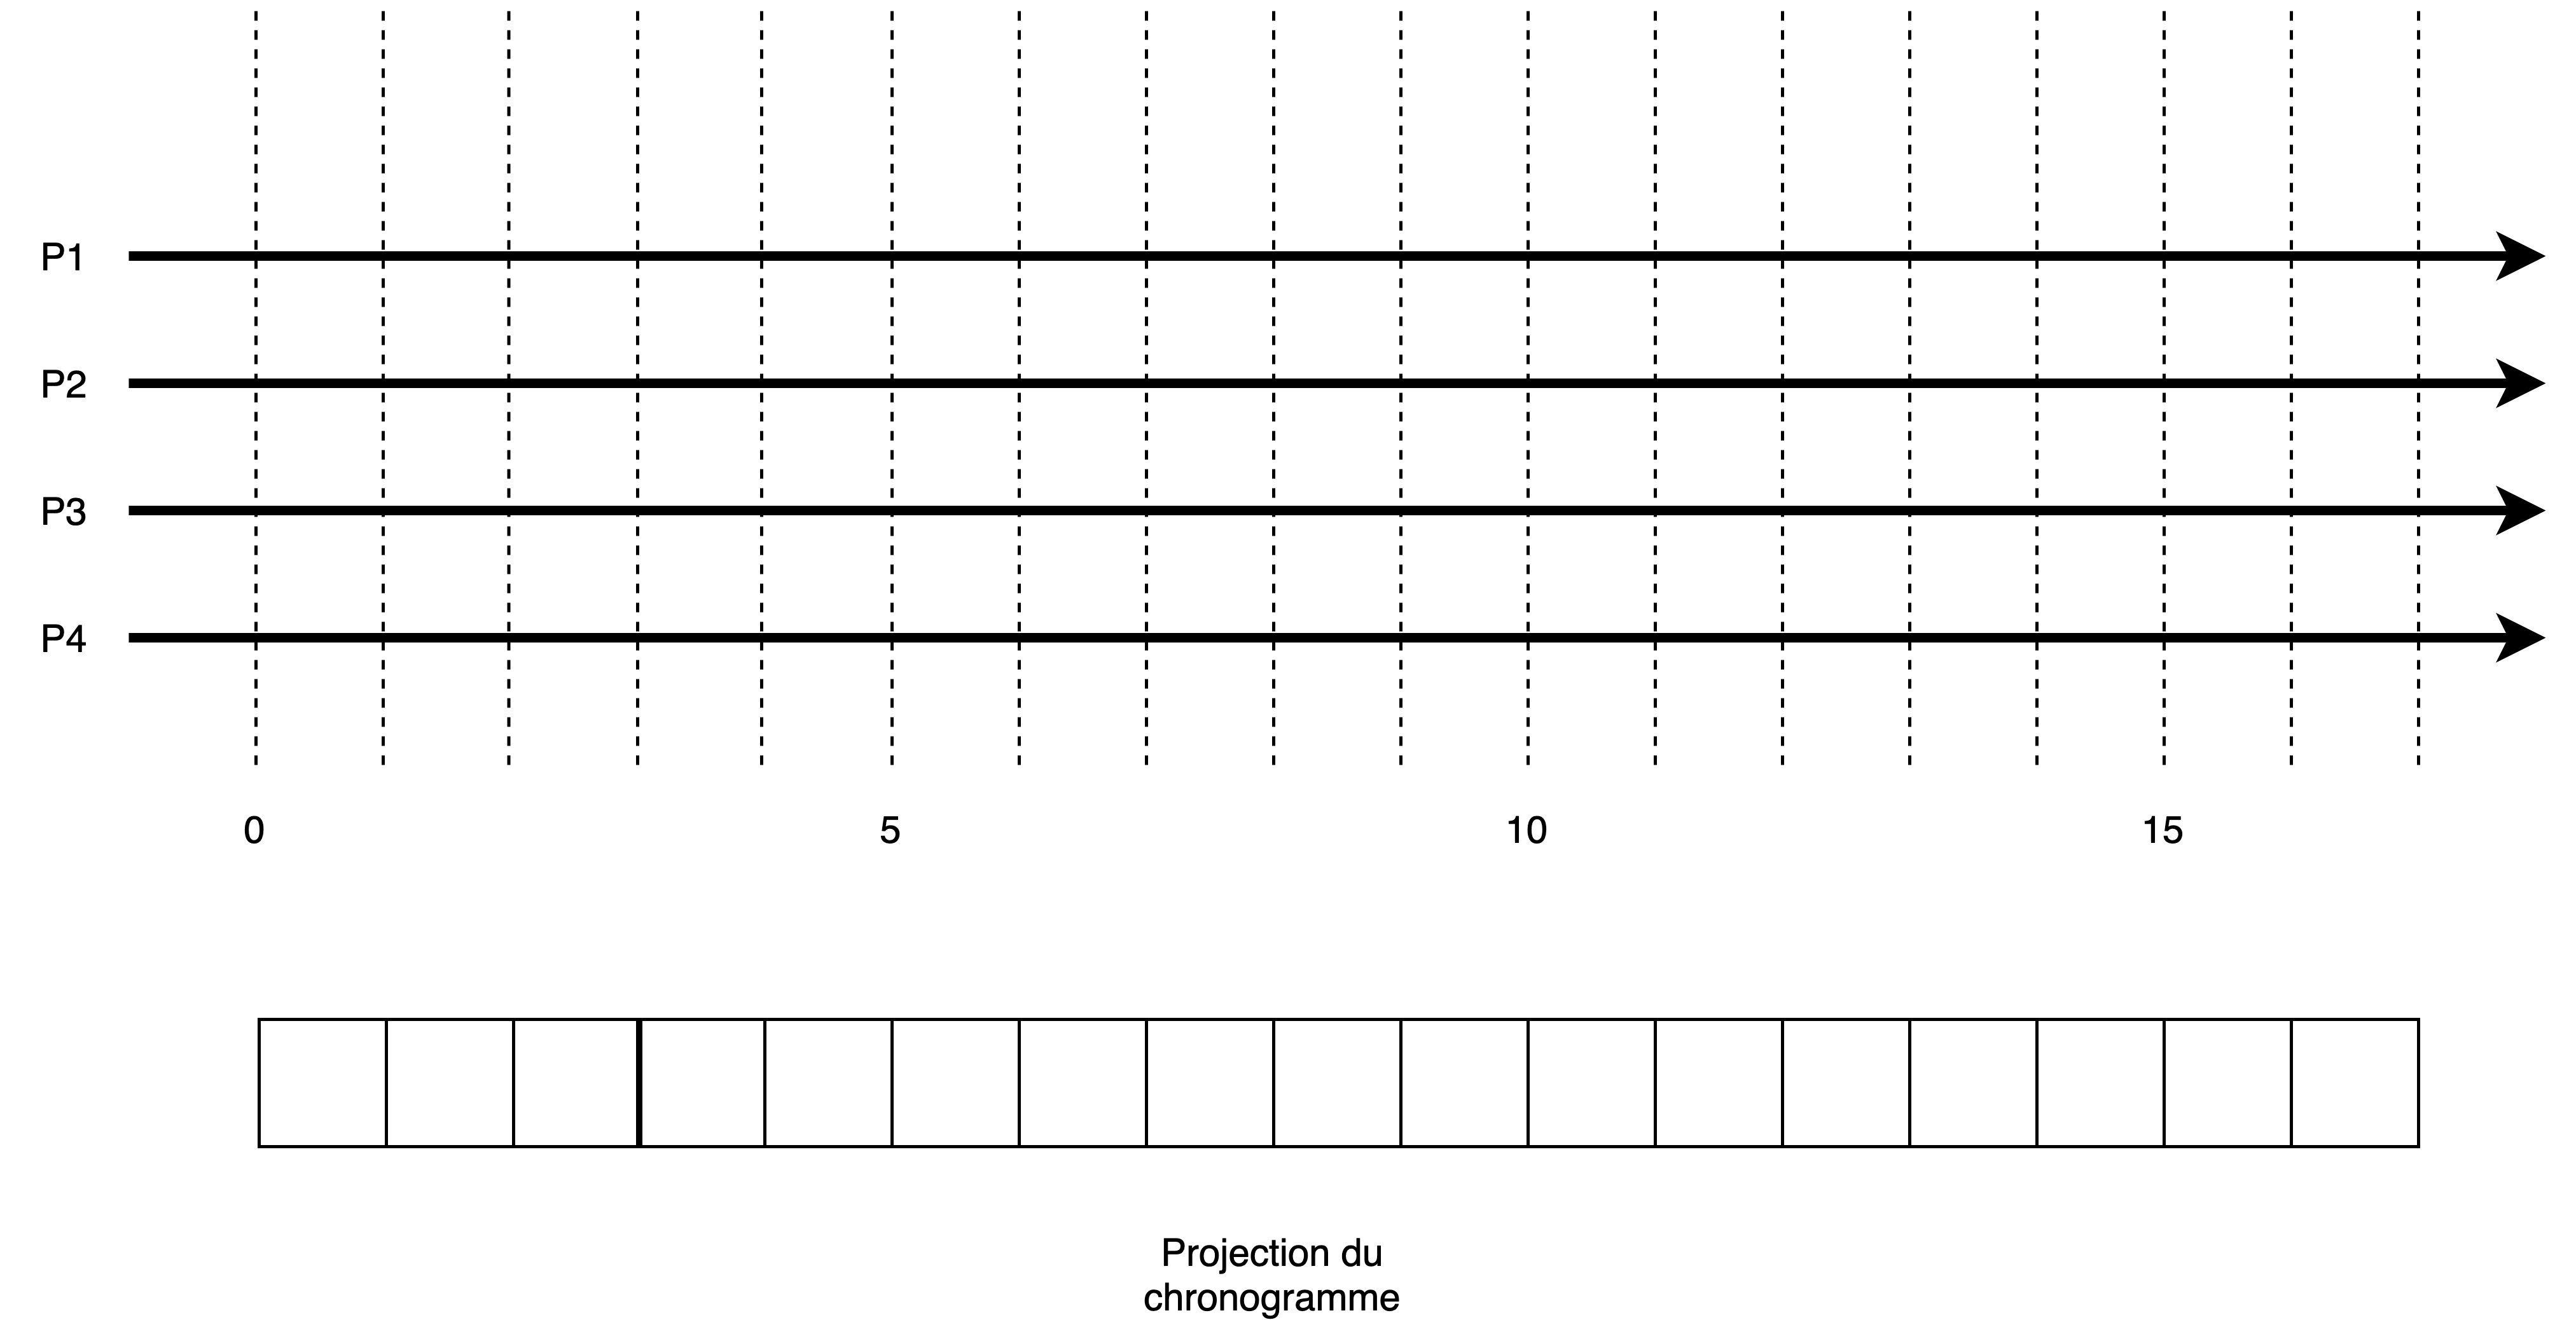
\includegraphics[width=10cm]{img/mc}\\
                     \end{center}
    \newpage
    
	\item 	SJF
    \begin{center}
                     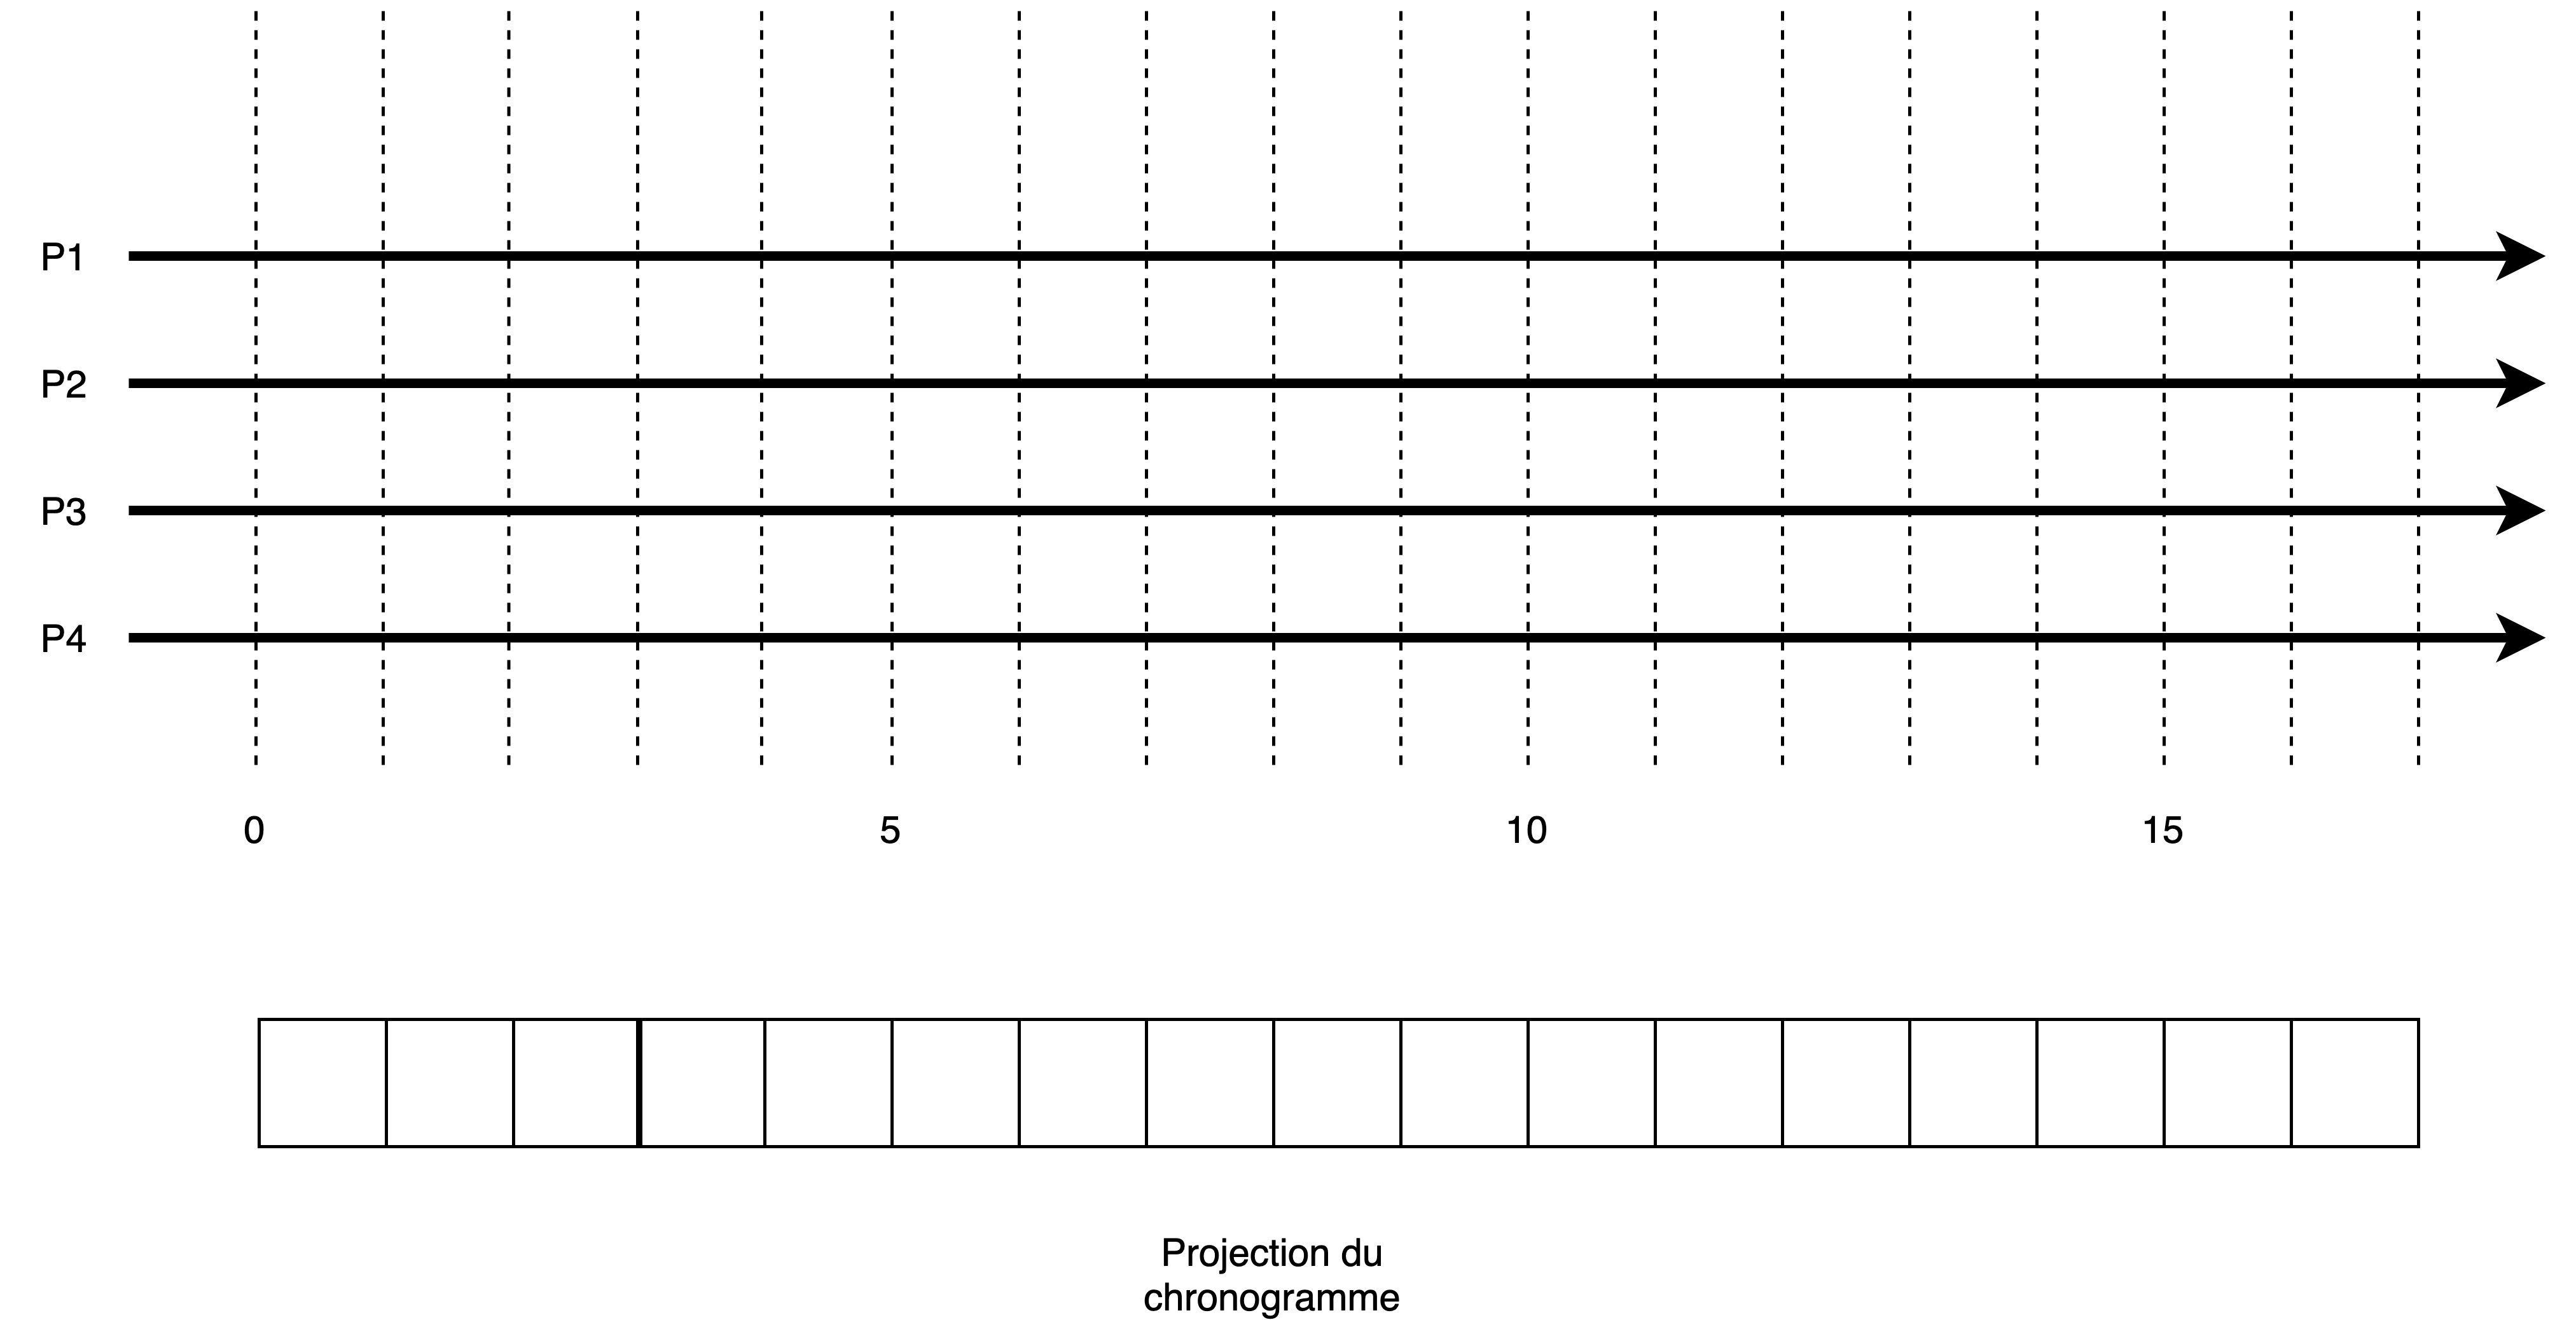
\includegraphics[width=10cm]{img/mc}\\
                     \end{center}
    \item SRJF
    \begin{center}
                     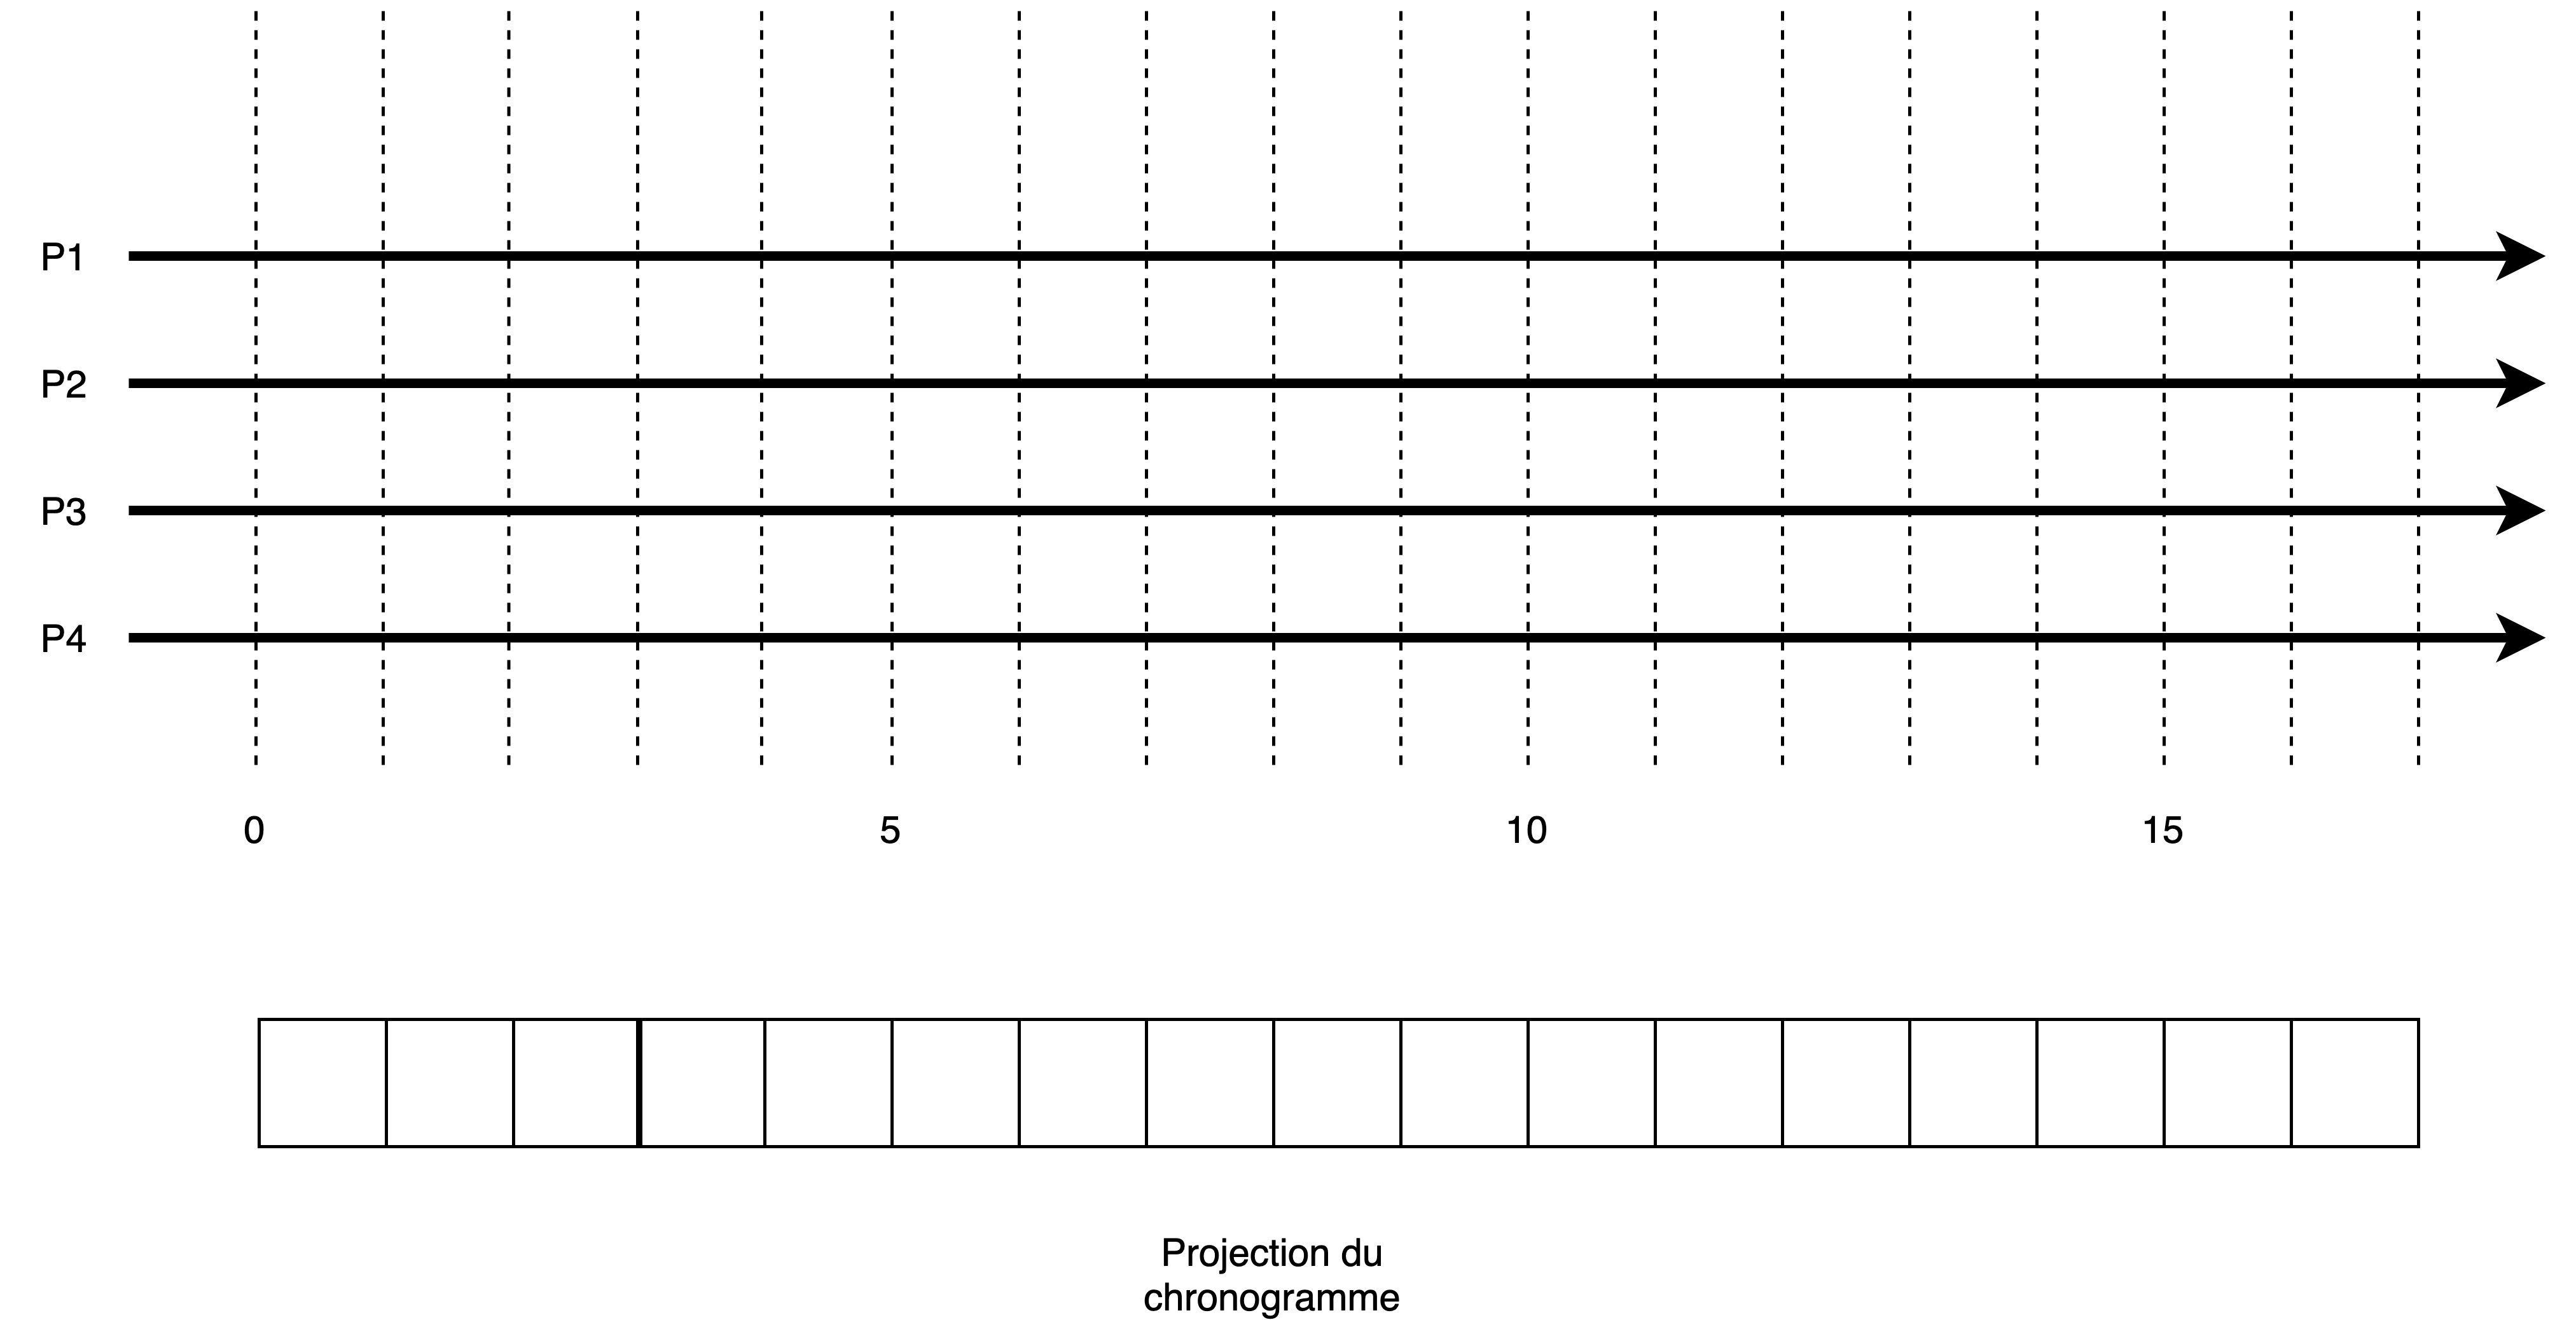
\includegraphics[width=10cm]{img/mc}\\
                     \end{center}
    \end{enumerate}
\end{document}